% SC3020 --- Chapter 8: Advanced Topics (0->100 ground-up)
\chapter{Advanced Topics: Text, Time Series, and Big Data}
\label{ch:advanced}

\begin{quote}
\emph{``Most of the world's data is text, ticks, and streams.''} We extend mining beyond tables to sequences, language, and data that never fits on one machine.
\end{quote}

\noindent\fbox{\parbox{\dimexpr\linewidth-2\fboxsep-2\fboxrule}{%
\textbf{From zero: no advanced data assumed.} We start from an SMS, a stock ticker, and a log stream, reformulate each as a mining problem, then formalise text representation, time-series motifs, and distributed computation. Pictures precede formalism.}}
\vspace{0.4em}

\section*{Learning Outcomes}
After this chapter you will be able to:
\begin{enumerate}[label=(L\arabic*)]
    \item transform text into numeric vectors (bag-of-words, TF-IDF, embeddings);
    \item describe time-series components and similarity (trend, seasonality, DTW);
    \item outline MapReduce/Spark execution and streaming sketches;
    \item explain scalability bottlenecks (shuffle, skew, velocity) and mitigations;
    \item scope an end-to-end project combining text/time-series at scale with ethical checks.
\end{enumerate}

% ============================================================
\section{Mining Text}
\label{sec:text}
\paragraph{Intuition.} ``I love this phone'' and ``I hate this phone'' differ by one word but opposite sentiment. Text must be turned into numbers that preserve discriminating patterns while discarding noise.

\paragraph{Bag-of-words pipeline.} Tokenisation (split on whitespace/punctuation, lower-case, handle emojis) $\to$ normalisation (stemming ``running''$\to$``run'', lemmatisation) $\to$ stop-word removal $\to$ vocabulary $V$ $\to$ vector $\mathbf{x}\in\mathbb{R}^{|V|}$ with term frequency $\text{tf}(t,d)$. Down-weight common words via inverse document frequency:
\begin{equation}
\text{idf}(t)=\log\frac{N}{\text{df}(t)},\qquad
\text{tf-idf}(t,d)=\text{tf}(t,d)\times\text{idf}(t),
\end{equation}
where $\text{df}(t)$ counts documents containing $t$. TF-IDF up-weights rare but document-specific terms. $n$-grams (pairs/triples) recover some order; embeddings (Word2Vec, contextual transformers) map words to dense vectors where cosine approximates meaning.

\begin{figure}[h]\centering
\begin{tikzpicture}[every node/.style={font=\scriptsize},
  b/.style={draw, thick, rounded corners=3pt, align=center, minimum width=2.0cm, minimum height=0.7cm}]
\node[b, fill=blue!12] (raw) at (0,0) {Raw text\\{\tiny SMS, review}};
\node[b, fill=orange!14] (tok) at (2.8,0) {Tokens\\{\tiny love, phone}};
\node[b, fill=green!14] (voc) at (5.6,0) {Vocabulary\\{\tiny $V$: 20k terms}};
\node[b, fill=violet!14] (vec) at (8.6,0) {TF-IDF vector\\{\tiny sparse $\mathbf{x}\in\mathbb{R}^{|V|}$}};
\node[b, fill=teal!12] (emb) at (8.6,-1.2) {Embedding\\{\tiny dense $\mathbf{e}\in\mathbb{R}^{300}$}};
\draw[-{Latex[length=2.5mm]}, thick, blue!60!black] (raw)--(tok);
\draw[-{Latex[length=2.5mm]}, thick, blue!60!black] (tok)--(voc);
\draw[-{Latex[length=2.5mm]}, thick, blue!60!black] (voc)--(vec);
\draw[-{Latex[length=2.5mm]}, thick, teal!60!black] (vec)--(emb) node[midway, right, font=\tiny, fill=teal!10, rounded corners=1pt, inner sep=1pt] {Word2Vec / BERT};
% bag diagram
\node[font=\tiny, fill=yellow!12, rounded corners=2pt, inner sep=2pt] at (4.3,-1.6) {order lost in BoW; $n$-grams or embeddings recover context};
\end{tikzpicture}
\caption{Text-to-vector pipeline. Bag-of-words treats documents as multisets of terms; TF-IDF reweights by informativeness; embeddings compress to dense semantics.}
\label{fig:text-pipeline}
\end{figure}

% ============================================================
\section{Time Series and Sequences}
\label{sec:timeseries}
\paragraph{Intuition.} A heart-rate trace has trend (rising), seasonality (daily cycle), and surprise (arrhythmia). Mining asks: what is expected, what deviates, and which traces look similar?

\paragraph{Formal view.} Time series $y_1,\dots,y_T$. Decomposition $y_t = T_t + S_t + R_t$ (trend + seasonal + residual) via moving averages or STL. Stationarity ($\mu,\sigma^2$ constant) is assumed by many models; differencing $\nabla y_t=y_t-y_{t-1}$ helps. Similarity: Euclidean requires equal length and alignment; \emph{Dynamic Time Warping} (DTW) allows warping: DTW$(Q,C)=\min_{\text{warp path }W}\sum_{(i,j)\in W}d(q_i,c_j)$ with monotonicity and boundary constraints (DP in $O(T^2)$, often pruned with LB-Keogh bounds). Motifs/discords: repeated/anomalous subsequences; forecasting (ARIMA, exponential smoothing) vs.\ classification (similarity-based or feature-based).

\begin{figure}[h]\centering
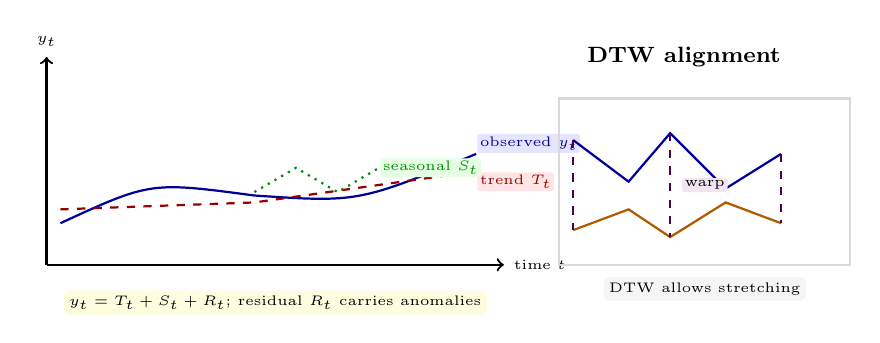
\begin{tikzpicture}[scale=0.88, every node/.style={font=\scriptsize}]
\draw[->, thick] (0,0)--(6.6,0) node[right, font=\tiny] {time $t$};
\draw[->, thick] (0,0)--(0,3.0) node[above, font=\tiny] {$y_t$};
% decomposition illustration
\draw[thick, blue!60!black] (0.2,0.6) .. controls (1.5,1.2) .. (3.0,1.0) .. controls (4.5,0.9) .. (6.2,1.6) node[above right, font=\tiny, fill=blue!10, rounded corners=1pt, inner sep=1pt] {observed $y_t$};
\draw[thick, red!60!black, dashed] (0.2,0.8) -- (3.0,0.9) -- (6.2,1.35) node[below right, font=\tiny, fill=red!10, rounded corners=1pt, inner sep=1pt] {trend $T_t$};
\draw[thick, green!55!black, dotted] (3.0,1.0) ++(0,0.05) -- ++(0.6,0.35) -- ++(0.6,-0.35) -- ++(0.6,0.35) node[right, font=\tiny, fill=green!10, rounded corners=1pt, inner sep=1pt] {seasonal $S_t$};
\node[font=\tiny, fill=yellow!12, rounded corners=2pt, inner sep=2pt] at (3.3,-0.55) {$y_t=T_t+S_t+R_t$; residual $R_t$ carries anomalies};
% DTW small second panel
\node[font=\footnotesize\bfseries] at (9.2,3.0) {DTW alignment};
\draw[thick, gray!30] (7.4,0) rectangle (11.6,2.4);
\draw[thick, blue!60!black] (7.6,1.8)--(8.4,1.2)--(9.0,1.9)--(9.8,1.1)--(10.6,1.6);
\draw[thick, orange!70!black] (7.6,0.5)--(8.4,0.8)--(9.0,0.4)--(9.8,0.9)--(10.6,0.6);
\foreach \i/\j in {1/1,2/2,3/3,4/4,5/5} {
  \pgfmathsetmacro{\xa}{7.6+(\i-1)*0.75}
  \pgfmathsetmacro{\xb}{8.4+(\j-1)*0.6}
  % simplified diagonal matching for illustration
}
\draw[dashed, violet!60!black, thick] (7.6,1.8)--(7.6,0.5);
\draw[dashed, violet!60!black, thick] (9.0,1.9)--(9.0,0.4);
\draw[dashed, violet!60!black, thick] (10.6,1.6)--(10.6,0.6);
\node[font=\tiny, fill=violet!10, rounded corners=1pt, inner sep=1pt] at (9.5,1.15) {warp};
\node[font=\tiny, fill=gray!8, rounded corners=2pt, inner sep=2pt] at (9.5,-0.35) {DTW allows stretching};
\end{tikzpicture}
\caption{Left: additive decomposition. Right: DTW aligns sequences by warping time (dashed) so similar shapes match despite speed/phase shifts.}
\label{fig:timeseries-dtw}
\end{figure}

% ============================================================
\section{Big Data and Streaming}
\label{sec:bigdata}
\paragraph{Intuition.} Data that does not fit on one machine, or never stops arriving, needs a different discipline: move computation to data, and answer from summaries/sketches.

\paragraph{MapReduce / Spark.} \emph{Map}: $(\text{key},\text{value})\mapsto\text{list}(k',v')$; \emph{shuffle/sort} by $k'$; \emph{Reduce}: $(k',\text{list}(v'))\mapsto\text{result}$. Fault-tolerant via replication and recomputation. Spark generalises to DAGs of RDDs/DataFrames with in-memory caching; DataFrame API and Catalyst optimiser made it practical. Key costs: \emph{shuffle} (network) and \emph{skew} (one key dominates --- mitigate by salting).

\paragraph{Streams.} Unbounded $x_1,x_2,\dots$ with one pass and sublinear memory. Sketches: Count-Min for frequency, HyperLogLog for cardinality, reservoir sampling for uniform sample, sliding windows with exponential decay. For mining on streams: incremental $k$-means, Hoeffding trees, and approximate FP-growth variants.

\begin{figure}[h]\centering
\begin{tikzpicture}[every node/.style={font=\scriptsize},
  b/.style={draw, thick, rounded corners=3pt, align=center, minimum width=2.2cm, minimum height=0.75cm}]
\node[b, fill=blue!12] (inp) at (0,0) {Input splits\\HDFS/S3};
\node[b, fill=orange!14] (map) at (3.0,0) {Map\\{\tiny tokenise, filter}};
\node[b, fill=green!14] (shuf) at (6.0,0) {Shuffle \& Sort\\{\tiny network heavy}};
\node[b, fill=violet!14] (red) at (9.0,0) {Reduce\\{\tiny sum, aggregate}};
\node[b, fill=red!12] (out) at (9.0,-1.4) {Output};
\draw[-{Latex[length=2.5mm]}, thick, blue!60!black] (inp)--(map);
\draw[-{Latex[length=2.5mm]}, thick, blue!60!black] (map)--(shuf);
\draw[-{Latex[length=2.5mm]}, thick, blue!60!black] (shuf)--(red);
\draw[-{Latex[length=2.5mm]}, thick, blue!60!black] (red)--(out);
% stream side
\node[b, fill=teal!12, minimum width=2.8cm] (stream) at (0,-1.4) {Stream $x_1,x_2,\dots$};
\node[b, fill=yellow!16, minimum width=2.8cm] (sketch) at (3.0,-1.4) {Sketch\\{\tiny Count-Min, HLL}};
\draw[-{Latex[length=2.5mm]}, thick, teal!60!black] (stream)--(sketch);
\draw[dashed, gray!60, thick] (sketch)--(shuf);
\node[font=\tiny, fill=yellow!12, rounded corners=2pt, inner sep=2pt] at (4.5,-2.2) {batch = MapReduce/Spark; \quad stream = one pass, $o(N)$ memory};
\end{tikzpicture}
\caption{Batch vs.\ stream. MapReduce/Spark scales by splitting and shuffling; streaming sacrifices exactness for bounded memory and real-time latency.}
\label{fig:mapreduce-stream}
\end{figure}

\begin{lstlisting}[language=Python, caption={Text + TF-IDF + classifier: a minimal sentiment pipeline.}, label={lst:text}]
from sklearn.feature_extraction.text import TfidfVectorizer
from sklearn.linear_model import LogisticRegression
from sklearn.pipeline import Pipeline

docs = ["I love this phone", "I hate this phone", "love love great", "hate terrible awful"]
y = [1,0,1,0]  # 1=positive, 0=negative
pipe = Pipeline([("tfidf", TfidfVectorizer(stop_words="english", ngram_range=(1,2))),
                ("clf", LogisticRegression())])
pipe.fit(docs, y)
print(pipe.predict(["love this great phone", "terrible hate"]))
print(pipe.named_steps["tfidf"].vocabulary_)
\end{lstlisting}

\begin{lstlisting}[language=Python, caption={MapReduce word count locally; then think distributed.}, label={lst:mapreduce}]
from collections import Counter
import itertools

# Map: emit (word,1) per document
def mapper(doc): return [(w.lower(),1) for w in doc.split()]

# Shuffle+Reduce: group by key and sum
docs = ["hello world", "hello data mining", "world of data"]
mapped = list(itertools.chain.from_iterable(mapper(d) for d in docs))
counts = Counter()
for k,v in mapped: counts[k]+=v
print(counts)  # Counter({'hello':2,'world':2,'data':2,'mining':1,'of':1})
# On Spark: sc.textFile("hdfs://...").flatMap(...).map(lambda w:(w,1)).reduceByKey(lambda a,b:a+b)
\end{lstlisting}

% ============================================================
\section{Putting It Together: An End-to-End Sketch}
\label{sec:project}
A production pipeline stitches chapters: CRISP-DM scoping (Ch.~1) $\to$ preprocessing and pipelines with no leakage (Ch.~2) $\to$ modelling (Ch.~3--6) $\to$ honest evaluation under imbalance (Ch.~7) $\to$ text/time-series features and scalable execution (this chapter). Add \emph{MLOps}: versioned data, reproducible pipelines, monitored drift, and ethical review (fairness, privacy, consent) at every stage. When data or the world shifts, the cycle repeats.

% ============================================================
% ============================================================
\section{Recommenders and Graph Mining at Scale}
\label{sec:recommender}
\paragraph{Collaborative filtering.} User-item matrix $R_{ui}$ (ratings or implicit clicks) is sparse. Latent-factor models factorise $R\approx P Q^\top$ where $\mathbf{p}_u,\mathbf{q}_i\in\mathbb{R}^k$ ($k\approx20$--$200$) and $\hat{r}_{ui}=\mathbf{p}_u^\top\mathbf{q}_i$. Optimise $\sum_{(u,i)\in\mathcal{K}}(r_{ui}-\mathbf{p}_u^\top\mathbf{q}_i)^2+\lambda(\|\mathbf{p}_u\|^2+\|\mathbf{q}_i\|^2)$ via SGD/ALS (Spark MLlib does this distributively). Neighbourhood models use item-item cosine on columns of $R$.

\paragraph{Graph mining.} Many big datasets are graphs (social, web, transaction). Tasks: community detection (Louvain --- modularity), PageRank (random-walk stationary), and pattern counting on edges. All motivate distributed graph engines (GraphX, Pregel) where computation moves to vertices.

\paragraph{Feature store and monitoring.} At scale, features are served from a \emph{feature store} (offline for training, online for serving) to prevent skew. Monitor data drift (PSI, KL) and concept drift (performance decay); automate retraining triggers but gate on ethical review --- especially when feedback loops recycle model predictions as future training data.

\begin{lstlisting}[language=Python, caption={ALS-style recommender intuition in pure Python (tiny demo).}, label={lst:als}]
import numpy as np
R = np.array([[5,3,0,1],[4,0,0,1],[1,1,0,5]], dtype=float)
mask = R>0
# trivial rank-2 ALS step (one iteration)
k=2
P = np.random.randn(3,k); Q = np.random.randn(4,k)
# fix Q, solve P row-wise (closed form for this demo: gradient step)
lr=0.01
for _ in range(200):
    pred = P @ Q.T
    err = (R - pred)*mask
    P += lr * (err @ Q)
    Q += lr * (err.T @ P)
print(np.round(P@Q.T,2))
\end{lstlisting}

% ============================================================
% ============================================================
\section{Ethics and MLOps for Advanced Data}
\label{sec:ethics-advanced}
\paragraph{Bias in text/time-series.} Word embeddings encode historical bias (``doctor'' closer to ``he'' than ``she''); time-series models trained on past regimes fail when regimes shift (COVID, market crash). Audit embeddings and stress-test temporal models on out-of-period data.

\paragraph{Privacy.} Text may contain PII; time series may be re-identifiable (heart trace). Techniques: differential privacy (add calibrated noise), $k$-anonymity for quasi-identifiers, and federated learning that keeps raw data on device.

\paragraph{MLOps loop.} Log data lineage, feature definitions, and model versions; monitor drift (PSI $>$ 0.2 triggers review); canary-deploy new models; require human approval for high-stakes actions. Ethics is not a final chapter --- it closes the CRISP-DM loop back to Business Understanding.

% ============================================================
\section{Chapter Notes}
Text: Manning, Raghavan \& Sch\"utze, \emph{Introduction to Information Retrieval} (2008) for TF-IDF; Mikolov et al. (2013) for Word2Vec. Time series: Hyndman \& Athanasopoulos, \emph{Forecasting} (2021); DTW: Berndt \& Clifford (1994). Big data: Dean \& Ghemawat (MapReduce, 2004); Zaharia et al. (Spark, 2012). Streaming sketches: Cormode \& Muthukrishnan (Count-Min).

% ============================================================
\section{Exercises}
\begin{enumerate}[label=E8.\arabic*, leftmargin=*, itemsep=0.6em]
    \item \textbf{TF-IDF.} Corpus of 3 docs, term ``data'' appears in 2 docs with tf $2,1,0$. Compute idf and tf-idf for doc 1. Why does a term in every document get zero idf?
    \item \textbf{DTW.} Sequences $Q=[1,2,3]$, $C=[1,2,2,3]$. Compute DTW distance with $d(q_i,c_j)=|q_i-c_j|$ by filling the DP matrix and tracing the optimal warp path.
    \item \textbf{MapReduce.} Design map and reduce for counting co-occurring item pairs within baskets. Where does skew arise and how would salting help?
    \item \textbf{Decomposition.} Sketch a series with linear trend $+$ yearly seasonality $+$ noise. Explain how differencing removes trend and why STL is preferred over a single moving average for seasonal extraction.
    \item \textbf{ Ethics at scale.} A streaming loan-approval model retrains nightly on recent data. Describe a failure mode where feedback loops amplify bias, and propose a monitoring metric and an intervention.
\end{enumerate}
% End of Chapter 8
